\documentclass[12pt]{article}

\usepackage{amsmath}
\usepackage{mathtools}
\usepackage{algorithm}

\usepackage{algorithmic}

\usepackage{enumitem}

\usepackage{amssymb}

\usepackage{graphicx}

\usepackage{hyperref}
\hypersetup{
    colorlinks=true,
    linkcolor=blue,
    filecolor=magenta,      
    urlcolor=cyan,
    bookmarks=true,
}
\usepackage[font=footnotesize]{caption}

\usepackage[utf8]{inputenc}
%\title{Recuit Simulé}
\begin{document}
    Le recuit simulé (\emph{Simulated annealing}), est une métaheuristique proposée par Kirkpatrick et al. [2] en1983. cette méthode est inspirée du recuit en métallurgie, une technique impliquant le chauffage et le refroidissement contrôlé d'un matériau pour augmenter la taille de ses cristaux et réduire leurs défauts. Les deux sont des attributs du matériau qui dépendent de son énergie thermodynamique. Le chauffage et le refroidissement du matériau affectent à la fois la température et l'énergie libre thermodynamique.

\subsection{Pseudocode}

\begin{algorithm}[H]
    \caption{Recuit simulé}
    \begin{algorithmic}
    \STATE Générer une solution initiale S aléatoirement. 
    \STATE Initialiser les paramètres Tinit , T0 et alpha 
    \STATE T$=$Tinit  (T: température courante)
    \WHILE{T$<$T0 and Time $<$ limite} 
        \STATE temperature de gel n'est pas atteinte et temps limite n'est pas dépassé
        \REPEAT{}
            \STATE Génerer un voisin S' $\in$ V(S) 
            \IF{F(S')$<=$ F(S)} 
                \STATE{S$=$S' \emph{//une meilleure solution a été trouvée} }
            \ELSE
                \STATE{S$=$S' avec une probabilité P de métropolis }
            \ENDIF
            \IF{f(S)$<$Best}
                \STATE{Best $=$ S \emph{//garder dans Best la meilleure solution en terme de nombre de boite utilisées. f(S) étant le nombre de boîtes utilisées par S.}}

            \ENDIF
        \UNTIL {R itérations or R/2 sans amélioration}
        \STATE{$T$=$ \alpha T $  \emph{//diminution de la température} }
    \ENDWHILE
     
\end{algorithmic}
\end{algorithm}

    L’algorithme du recuit simulé pour le problème du bin packing est donné ci-dessus.
 L’algorithme commence par une température initiale \emph{$T_{init}$}, cette température est progressivement diminuée par un facteur $\alpha$ jusqu'à l’atteinte d’un seuil minimal \emph{$T_{0}$} ( Température de Gel). 
Dans chaque température T, le système (solution actuelle) est perturbé plusieurs fois (R fois). 
l’algorithme commence par une solution initiale S (affectation des articles aux boîtes), 
cette solution est générée aléatoirement, à chaque itération une solution voisine S’ est générée aléatoirement en utilisant le processus expliqué dans la partie (\emph{1.1.3 Génération des voisins}) . 
la valeur de la fonction objective $F (S’)$ est calculée. 
Si le voisin S’ a amélioré la valeur de la fonction objective ($ F(S’)> F(S)$)  , 
la solution S’ est acceptée comme la nouvelle solution ( S$= $S’) , sinon, elle est acceptée selon la probabilité de métropolis \newline

$ P_{acceptation}(S') = e^{\frac{F(S')-F(S)}{T}}$ \newline



L’algorithme s'arrête quand la température \emph{$T_{0}$} est atteinte, et retourne la meilleure solution trouvée,
 dans cette étape on prend la meilleure solution en terme de nombre de boîtes utilisées (gardée dans la variable Best). 

\subsubsection{Critère d'arrêt}
L’algorithme s’arrête quand la température de gel \emph{$T_{0}$} est atteinte, et dans chaque température T le processus de recherche de voisinage est exécuté R fois.

\subsubsection{Fonction objective}
La fonction objective est utilisée pour accepter une solution voisine S’ = V(S), elle est donnée par la formule suivante : 
\begin{equation}
    \max{F(S')} = \sum_{i=1}^m (\sum_{j=1}^{k_{i}} w_{j})^{2}
\end{equation}
avec : 
\begin{itemize}
\item \(m\) : nombre de boîtes utilisées dans S’ 
\item \(k_i\) : nombre d’articles rangés dans la boîte i 
\item \(w_j\) : le volume de l’article j 
\end{itemize}
Cette fonction permet de maximiser le taux de remplissage des boîtes utilisées dans la solution ce qui va nous mener vers une meilleure solution en terme de nombre de boîtes utilisées. 

la raison de ne pas avoir utilisé la fonction objective définie dans le problème du bin packing ( minimiser le nombre de boîtes utilisées) est que cette dernière donne la même valeur pour plusieurs solutions différentes et ne montre pas les changements au niveau du contenu des boîtes. 

\subsubsection{Génération des voisins}
Pour chercher de nouvelles solutions à partir d’une solution S, l’algorithme utilise l’une des 2 techniques: Swap (0,1) , Swap (1,1). 
\begin{itemize}
    \item Swap(0,1): Consiste à déplacer un article choisi aléatoirement d’une boite à une autre 
    en maximisant la fonction objective (ie augmenter le remplissage des boîtes). 
    Il a été montré que cette technique est efficace dans les hautes températures ($T>=T_{1/2}$) avec $ T_{1/2} = \frac{T_{init}+T_{0}}{2}$ 
    \item Swap(1,1): Consiste à permuter entre 2 articles choisis aléatoirement et qui sont dans 2 boîtes différentes, en maximisant la fonction objective (ie augmenter le remplissage des boîtes).
     Il a été montré que cette technique est efficace dans les basses températures ($T<T_{1/2}$)
\begin{figure}[H]
    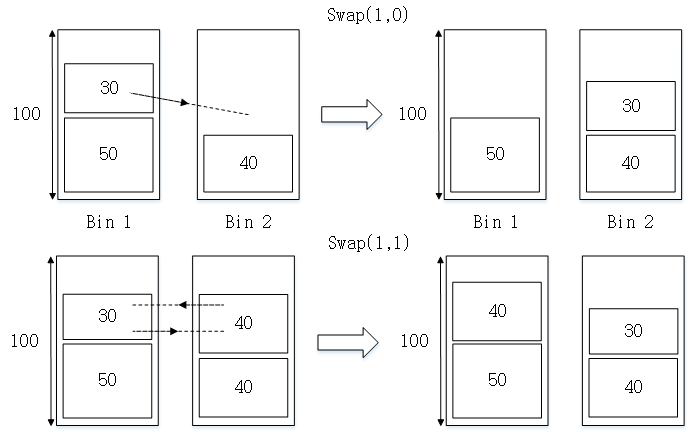
\includegraphics[width=\linewidth]{../figures/RS_SWAP.png}
    \caption{fonctions swap(1,0) et swap (1,1)}
    \label{fig:swap}
\end{figure}
\end{itemize}
\subsection{Les paramètres du recuit simulé }
\subsubsection{Le nombre d'itérations R}
Signifie le nombre de fois à faire une recherche locale avant de diminuer la température. Dans notre cas cette valeur est fixée par calibrage de paramètres à $R = 1000$.
 De plus la boucle peut s’arrêter si après $R/2$ itérations on n'obtient aucune amélioration.
\subsubsection{La température T}
La température T décroît au cours des itérations et influe d’une façon directe sur la probabilité d’acceptation des solutions non améliorantes: 
\begin{itemize}
    \item Premières itérations : T elevée $\implies $ acceptation fréquente des solutions non améliorantes (Diversification)
    \item Dernières itérations : T faible $\implies $ acceptation rare des solutions non améliorantes (Intensification) 
    
\end{itemize}

\subsubsection{Valeur de Tinit}
La valeur initiale Tinit doit permettre d’accepter initialement la plupart des solutions voisines (Diversification), généralement elle est fixée pour avoir une probabilité d’acceptation p0 de 0.8. 
La valeur de la température initiale Tinit dépends de la fonction objective et de l’instance du problème. Dans notre cas elle est estimée en effectuant une recherche initiale en acceptant toute les solutions générées, et en calculant la moyenne des différences dans la fonction objective, elle est donnée donc par la formule suivante : 

\begin{equation}
    T_{init} = \frac{|\Delta F|}{\ln p_{0}}
\end{equation}
\subsubsection{Valeur de T0}
Cette valeur définie le nombre d’itération à effectuer, elle doit être suffisamment petite pour atteindre l’état de gèle, dans notre cas, elle est fixée à 0.1, mais l’algorithme peut s’arrêter si les conditions suivantes sont vérifiées: 
\begin{itemize}
    \item Pas d’amélioration trouvée durant les R itérations d’une température T
    et la probabilité d’acceptation est assez petite ($<0.01$).
    \item Le temps d'exécution limite est atteint.
\end{itemize}

\subsubsection{Le facteur de diminution de la températures}
Ce facteur définit le schéma de refroidissement de notre système, c’est à dire la vitesse de convergence vers la solution finale.  sa valeur est généralement  entre 0.8 et 1.
\begin{itemize}
    \item Si $ \alpha $ est très grand, la convergence est trop rapide, dans ce cas on aura une convergence prématurée (on reste dans un optimum local).
    \item Si $ \alpha $ est très petit , la convergence est trop lente, dans ce cas on aura une exploration trop importante (temps d'exécution très élevé).
Après calibrâge de paramètres, cette valeur est fixée à 0.925.    
\end{itemize}

\subsection{Tests et résultats }
Dans cette partie on présentera les résultats d'exécution de notre méthode du recuit simulé avec les paramètres défini précédemment \textbf{$R=1000,T_{0}=0.1,\alpha =0925$}.
Le tableau dans \textbf{ \emph{figure \refeq{tab:texec}} } montre le temps d'exécution moyen de chaque type d’instance 
( la moyenne d'exécution de 5 instances de même type)  par la métaheuristique recuit simulé.

\begin{figure}[H]
    \centering
    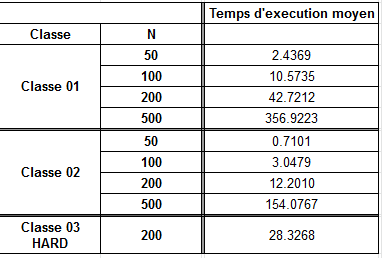
\includegraphics[]{../figures/RS/rs tab temps.PNG}
    \caption{tableau des temps d'exécution moyens du recuit simulé}
    \label{tab:texec}
\end{figure}
L’histogramme \textbf{\emph{figure \refeq{fig:texec}}} présente les temps d’exécutions  du recuit simulé en fonction des instances.
\begin{figure}[H]
    \centering
    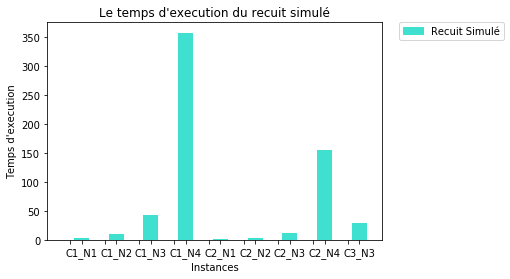
\includegraphics[width=\linewidth]{../figures/RS/texec rs(1).png}
    \caption{histogramme des temps d'execution du recuit simulé}
    \label{fig:texec}
\end{figure}
La  \textbf{\emph{figure \refeq{fig:n_bins}}} compare le nombre de boîtes obtenu par le recuit simulé avec la solution optimale
\begin{figure}[H]
    \centering
    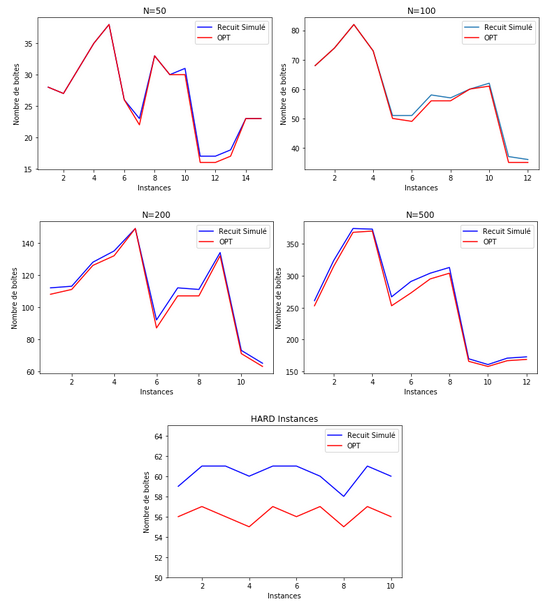
\includegraphics[width=\linewidth, scale=1.3]{../figures/RS/rs figures.PNG}
    \caption{le nombre de boites obtenues par le recuit simulé par rapport à la solution optimale}
    \label{fig:n_bins}
\end{figure}
Dans le tableau et le graphe \textbf{\emph{figure \refeq{fig:ratio}}}on donne la qualité de solution obtenue par le recuit simulé en utilisant la métrique du worse case ratio.
\begin{figure}[H]
    \centering
    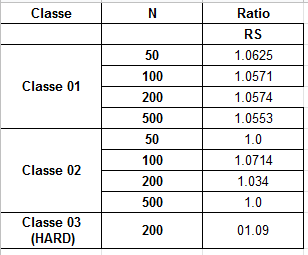
\includegraphics[scale=1]{../figures/RS/rs tab ratio.PNG}
    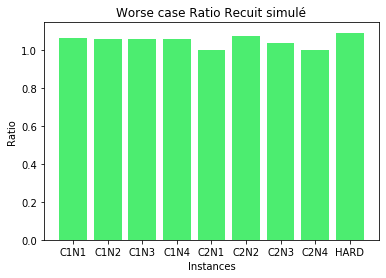
\includegraphics[scale=0.8]{../figures/RS/ratio RS.png}
    \caption{worse case ratio du recuit simulé}
    \label{fig:ratio}
\end{figure}
 
\subsubsection{Analyse et interprétation des résultats}
\begin{itemize}
    \item Le temps d’exécution du recuit simulé est très élevé, même avec les plus petites instances. 
    \item Ce temps d’exécution augmente avec la taille du problème et varie de \emph{0.7s} pour N=50 (classe 2) , jusqu’à \emph{357s} pour N=500 (classe1),[\textbf{\emph{figure \refeq{tab:texec}}} , \textbf{\emph{figure \refeq{fig:texec}}}].
    \item le temps d’exécution correspond à l’exécution 10 fois du Recuit simulé, ceci était nécessaire à cause de la nature stochastique de l’algorithme,  la solution initiale générée aléatoirement et la variable aléatoire \emph{u} utilisée pour accepter la solution non améliorante, influent sur les résultats obtenus.
    \item En terme de qualité de solution, le recuit simulé est capable de délivrer une bonne qualité de résultats pour le Scholl Benchmark, il arrive souvent à trouver la solution optimale pour les 2 premières classes du benchmark, et un peu moins pour la 3ème classe. [\textbf{\emph{figure \refeq{fig:n_bins}}}]
    \item Le Ratio obtenu par le recuit simulé est proche de 1 dans la plupart des cas, sauf dans le cas N=4 de la 1ere classe (C1N4), où on remarque une petite augmentation du ratio. 
    \item Cela signifie qu’on a pas une grande déviation par rapport à la solution optimale, donc d’une façon générale, le recuit simulé fournit une bonne qualité de résultats même dans le pire des cas (les instances les plus difficiles), avec une qualité un peu moins bonne dans les instances C1N4.On justifie cette dégradation par la taille de ces instances (N4=500 objets), le temps limité accordé au recuit simulé n’est pas suffisant pour lui permettre de bien explorer l’espace de recherche. 

\end{itemize}
\end{document}